\documentclass{article}

% if you need to pass options to natbib, use, e.g.:
%     \PassOptionsToPackage{numbers, compress}{natbib}
% before loading neurips_2019

% ready for submission
% \usepackage{neurips_2019}

% to compile a preprint version, e.g., for submission to arXiv, add add the
% [preprint] option:
%     \usepackage[preprint]{neurips_2019}

% to compile a camera-ready version, add the [final] option, e.g.:
     \usepackage[final]{neurips_2019}

% to avoid loading the natbib package, add option nonatbib:
%     \usepackage[nonatbib]{neurips_2019}

\usepackage[utf8]{inputenc} % allow utf-8 input
\usepackage[T1]{fontenc}    % use 8-bit T1 fonts
\usepackage{hyperref}       % hyperlinks
\usepackage{url}            % simple URL typesetting
\usepackage{booktabs}       % professional-quality tables
\usepackage{amsfonts}       % blackboard math symbols
\usepackage{nicefrac}       % compact symbols for 1/2, etc.
\usepackage{microtype}      % microtypography
\usepackage{graphicx}
\usepackage{subfig}
\usepackage{algpseudocode,algorithm}

\title{Implementing GAN on MNIST and SVHN}

% The \author macro works with any number of authors. There are two commands
% used to separate the names and addresses of multiple authors: \And and \AND.
%
% Using \And between authors leaves it to LaTeX to determine where to break the
% lines. Using \AND forces a line break at that point. So, if LaTeX puts 3 of 4
% authors names on the first line, and the last on the second line, try using
% \AND instead of \And before the third author name.

\author{%
  Shengjie Sun \\
  ss5593\\
  Department of Statistics\\
  Columbia University\\
  New York, NY 10027 \\
  \texttt{ss5593@columbia.edu} \\
  % examples of more authors
  \And
  Zeyu Yang \\
  zy2327 \\
  Department of Statistics\\
  Columbia University\\
  New York, NY 10027 \\
  \texttt{zy2327@columbia.edu}
  % \AND
  % Coauthor \\
  % Affiliation \\
  % Address \\
  % \texttt{email} \\
  % \And
  % Coauthor \\
  % Affiliation \\
  % Address \\
  % \texttt{email} \\
  % \And
  % Coauthor \\
  % Affiliation \\
  % Address \\
  % \texttt{email} \\
}

\begin{document}

\maketitle

\begin{abstract}
  We implement DCGAN on MNIST and SVHN dataset.
  The generated samples for both datasets are great although it takes quite some time to train the model.
  To help the model converge faster, we implement WGAN as well.
  The result \textbf{TBD}.
\end{abstract}

\section{Introduction}

Generative Adversarial Nets (GAN), first introduced by Ian Goodfellow in 2014[1], is a model that can be used to generate new images. 
It has been a hot topic since then.

The core idea of GAN is to create a two-player game. 
Build a generator that creates fake images while the discriminator tells whether the image is true or fake.

We train $D$ to maximize the probability of assigning the
correct label to both training examples and samples from G. 
We simultaneously train G to minimize $log(1-D(G(z)))$.

The optimum case is that the generate can fully recover the distribution of the data and the discriminator cannot tell whether the image is fake or not i.e. the output of discriminator is $1/2$.

\section{Implementation on MNIST}

MNIST dataset is a dataset of handwritten images, including 60,000 training images and 10,000 testing images.
All digits have been size-normalized and centered in a $28\times 28$ fixed-size image[2].

The dataset has been generally used to conduct pattern recognition. 
In this project, however, we will use the training image to train our GAN model and generate similar images.

\subsection{Architecture}

We used Deep Convoltional GAN (DCGAN)[4] as our structure. 
It has plenty convolutional layers and does not have max pooling layer.
We mainly use transpose convolutional layer to perform upsampling in our model.

\subsubsection{Generator}

The input of the first dense layer the $100\times 1$ random noise vector. 
We have $12,544$ neurons, apply batch normalization and activation function Leaky Relu, and reshape it to $7\times 7\times 256$.

The second Convoltional Transpose layer outputs $7\times 7\times 128$.

The third and fourth Convolutional layers have stride 2 and padding \textit{same}, they alter the first two dimensions of the input and make the input from $7\times 7$ to $14\times 14$ to $28\times 28$.
The filter makes the third dimension from 128 to 64 to 1.

Thus the final output is a $28\times 28\times 1$ black and white image.

\begin{itemize}
  \item First layer: Dense
    \begin{itemize}
      \item Input: $100 \times 1$ vector
      \item Units: $12,544$
      \item Batch normalization
      \item Activation: leaky relu
      \item Reshape $12,544$ to $7\times 7\times 256$
    \end{itemize}
  \item Second layer: Conv2DTranspose
    \begin{itemize}
      \item Input $7\times 7\times 256$
      \item Filter: 128
      \item Kernel size: 5
      \item Stride: 1
      \item Padding: same
      \item Batch normalization
      \item Activation: leaky relu
  \end{itemize} 
  \item Third layer: Conv2DTranspose
    \begin{itemize}
      \item Input $7\times 7\times 128$
      \item Filter: 64
      \item Kernel size: 5
      \item Stride: 2
      \item Padding: same
      \item Batch normalization
      \item Activation: leaky relu
    \end{itemize}   
  \item Fourth layer: Conv2DTranspose
    \begin{itemize}
      \item Input $14\times 14\times 64$
      \item Filter: 1
      \item Kernel size: 5
      \item Stride: 2
      \item Padding: same
      \item Activation: tanh
      \item Output $28\times 28\times 1$
    \end{itemize}   
\end{itemize}

\subsubsection{Discriminator}

The discriminator takes in a $28\times 28\times 1$ array. After three convolutional layers and one dense layer, the output will be a scalar.
This scalar will be applied to a logistics function in future steps to be a probability that lies between 0 and 1. It is the probability of the input being a true image or a fake image.

\begin{itemize}
  \item First layer: Conv2D
    \begin{itemize}
      \item Input: $28 \times 28\times 1$ array
      \item Filter: 64
      \item Kernel size: 5
      \item Stride: 2
      \item Padding: same
      \item Activation: leaky relu
      \item Dropout: 0.3
  \end{itemize} 
  \item Third layer: Conv2D
    \begin{itemize}
      \item Filter: 128
      \item Kernel size: 5
      \item Stride: 2
      \item Padding: same
      \item Activation: leaky relu
      \item Dropout: 0.3
    \end{itemize}   
  \item Fourth layer: Conv2D
    \begin{itemize}
      \item Filter: 256
      \item Kernel size: 5
      \item Stride: 2
      \item Padding: same
      \item Activation: leaky relu
      \item Dropout: 0.3
    \end{itemize} 
  \item Fifth layer: Flatten
  \item Sixth layer: Dense with output 1
\end{itemize}

\subsubsection{Hyperparameters}

\begin{itemize}
  \item Epoch: 100
  \item Batch: 256
  \item Learning rate
    \begin{itemize}
      \item Generator: 1e-3
      \item Discriminator: 1e-4
    \end{itemize}
\end{itemize}

We have experimented on different bacthes and epoches and we believe a batch of 256 samples and 100 epoches already produced satisfying result. 
In fact, the quality of the image does not seem to have significant improve after 50 epoches.

The reason why we choose the learning rate for the discriminator 10 times smaller than the learning rate for generator is 
because we noticed the loss of discriminator is much smaller than the loss of generator. 
To avoid the gradient jumping back and forth around the optimum spot, we lower the learning rate for discriminator.
The training result shows that the loss for both of them are at the same magnitude after the modification.

\subsection{Result}

\subsubsection{Tensorboard}

\begin{figure}[!htb]
  \centering
  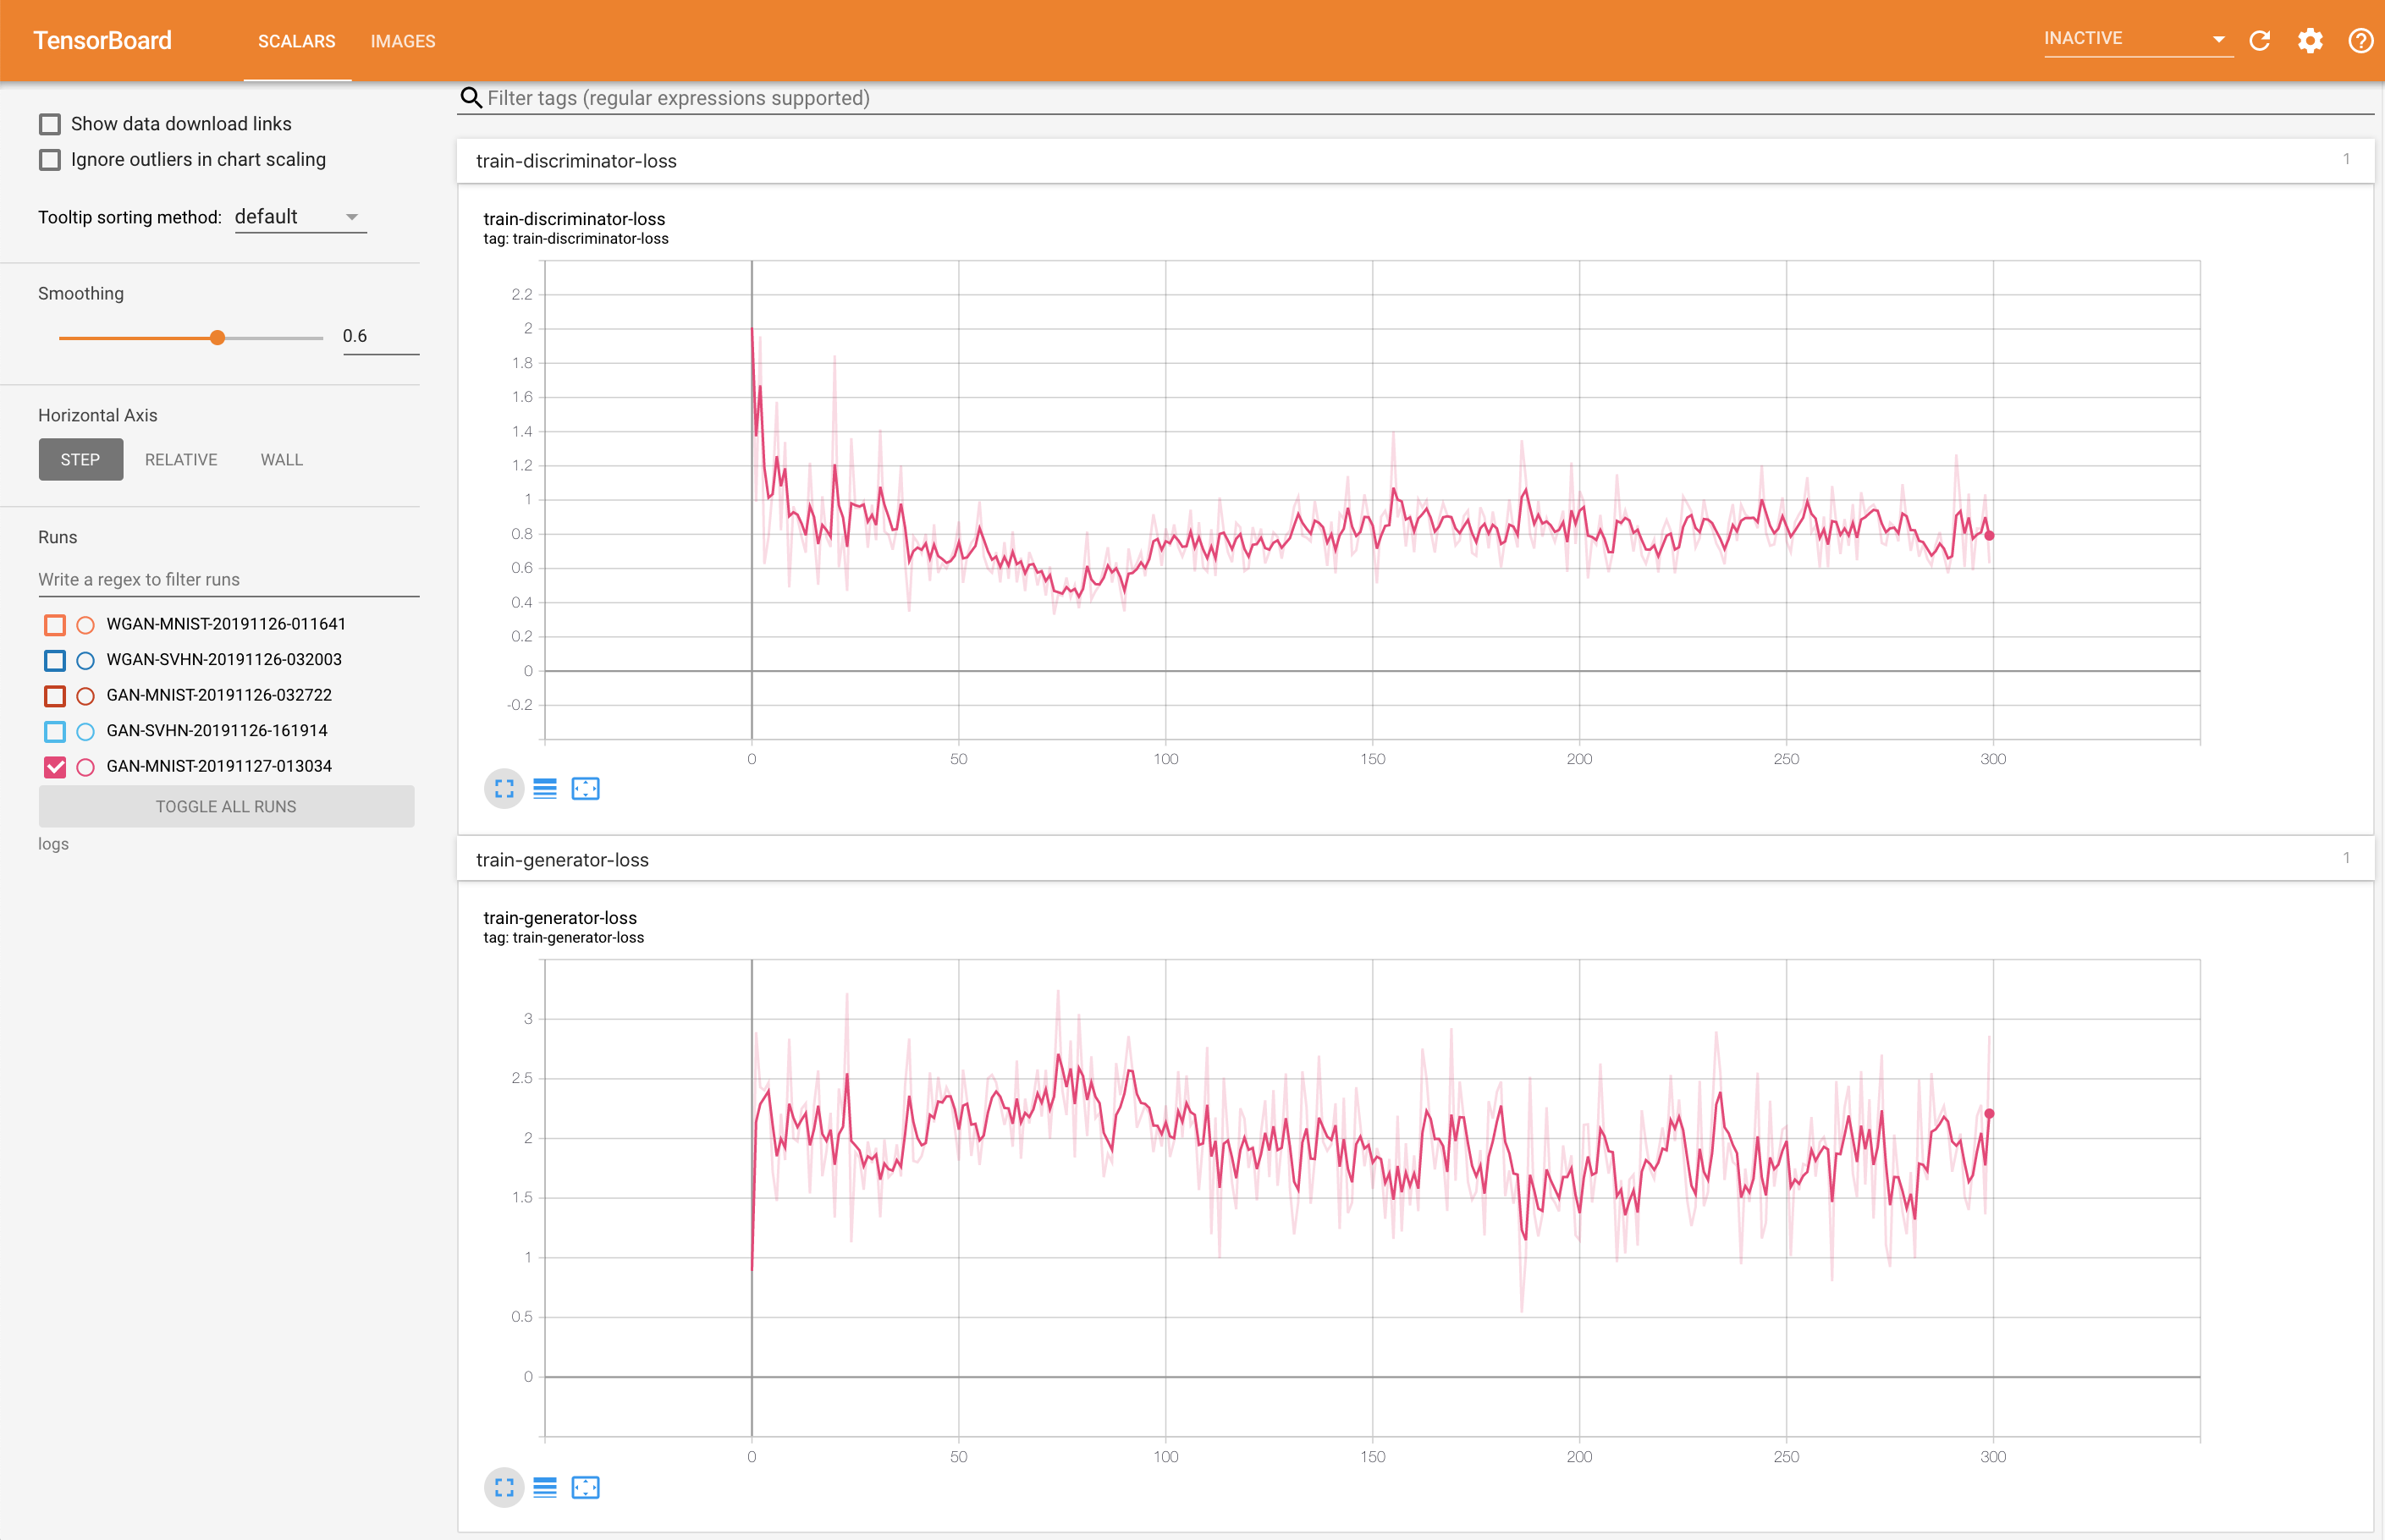
\includegraphics[width=0.8\textwidth]{tensorboard-GAN-MNIST.png}
  \caption{Tensorboard GAN MNSIT}
  \label{fig:TB_GAN_MNSIT}
\end{figure}

As we can observe from Figure~\ref{fig:TB_GAN_MNSIT}, training loss of both generator and discriminator is fluctuating. 
And generally when the loss of generator decreases, the loss of discriminator increases. This is the representation of the two player game i.e. both players want to minimize their own loss.

Although the loss remains around the same level and does not continue decrease, the quality of the images are in fact improving as we can see in the following section.

\subsubsection{Generated samples}

\begin{figure}[!htb]
  \centering
  \subfloat[MNIST data]{
  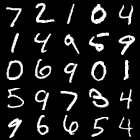
\includegraphics[width=0.2\textwidth]{mnist_data.png}}
  \subfloat[Epoch 10/100]{
  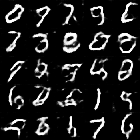
\includegraphics[width=0.2\textwidth]{I1.png}}
  \subfloat[Epoch 30/100]{
  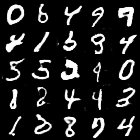
\includegraphics[width=0.2\textwidth]{I2.png}}
  \subfloat[Epoch 100/100]{
  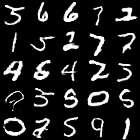
\includegraphics[width=0.2\textwidth]{I4_after-296-batches.png}}
  \caption{Comparison of MNIST data and generated samples from DCGAN}
  \label{fig:DCGAN_MNIST}
\end{figure}

From Figure ~\ref{fig:DCGAN_MNIST}, 
we can see the generated samples has a good approximation after 30 epoches.

The samples from the 10th are quite blury and they cannot have a good representation of number 2, 5, 8, etc.

The latter samples are clearer and the edges of the numbers are smoother. Number 0, 1, 3, 5, 7, 9 are quite ideal.

Although not all samples are of high quality, there are a proportion of the images that have the quality of the samples presented in paper[1] 2(a).

\section{Implementation on SVHN}

SVHN dataset is a dataset similar to MNIST, containing real-world digit images that obtained from house numbers in Google Street View images.
The images have been cropped into $32\times 32$ fixed-size array with three channels.

In this project, we will again use the training image to train our GAN model and generate similar images.

\subsection{Architecture}

\subsubsection{Generator}

The generator is slightly modifed from the generator for MNIST. 
The output of the first dense layer is changed to $8\times 8\times 256$ 
and the filter of the fourth layer (Conv2DTranspose) has changed from 1 to 3
so that the output of the whole generator would be a $32\times 32\times 3$ image.

\subsubsection{Discriminator}

Discriminator is exactly the same as the previous one.

\subsubsection{Hyperparameters}

\begin{itemize}
  \item Epoch: 200
  \item Batch: 256
  \item Learning rate
    \begin{itemize}
      \item Generator: 1e-3
      \item Discriminator: 1e-4
    \end{itemize}
\end{itemize}

Since the SVHN dataset is more complicated, we train the model with 200 epoches.

\subsection{Result}

\subsubsection{Tensorboard}

\begin{figure}[!htb]
  \centering
  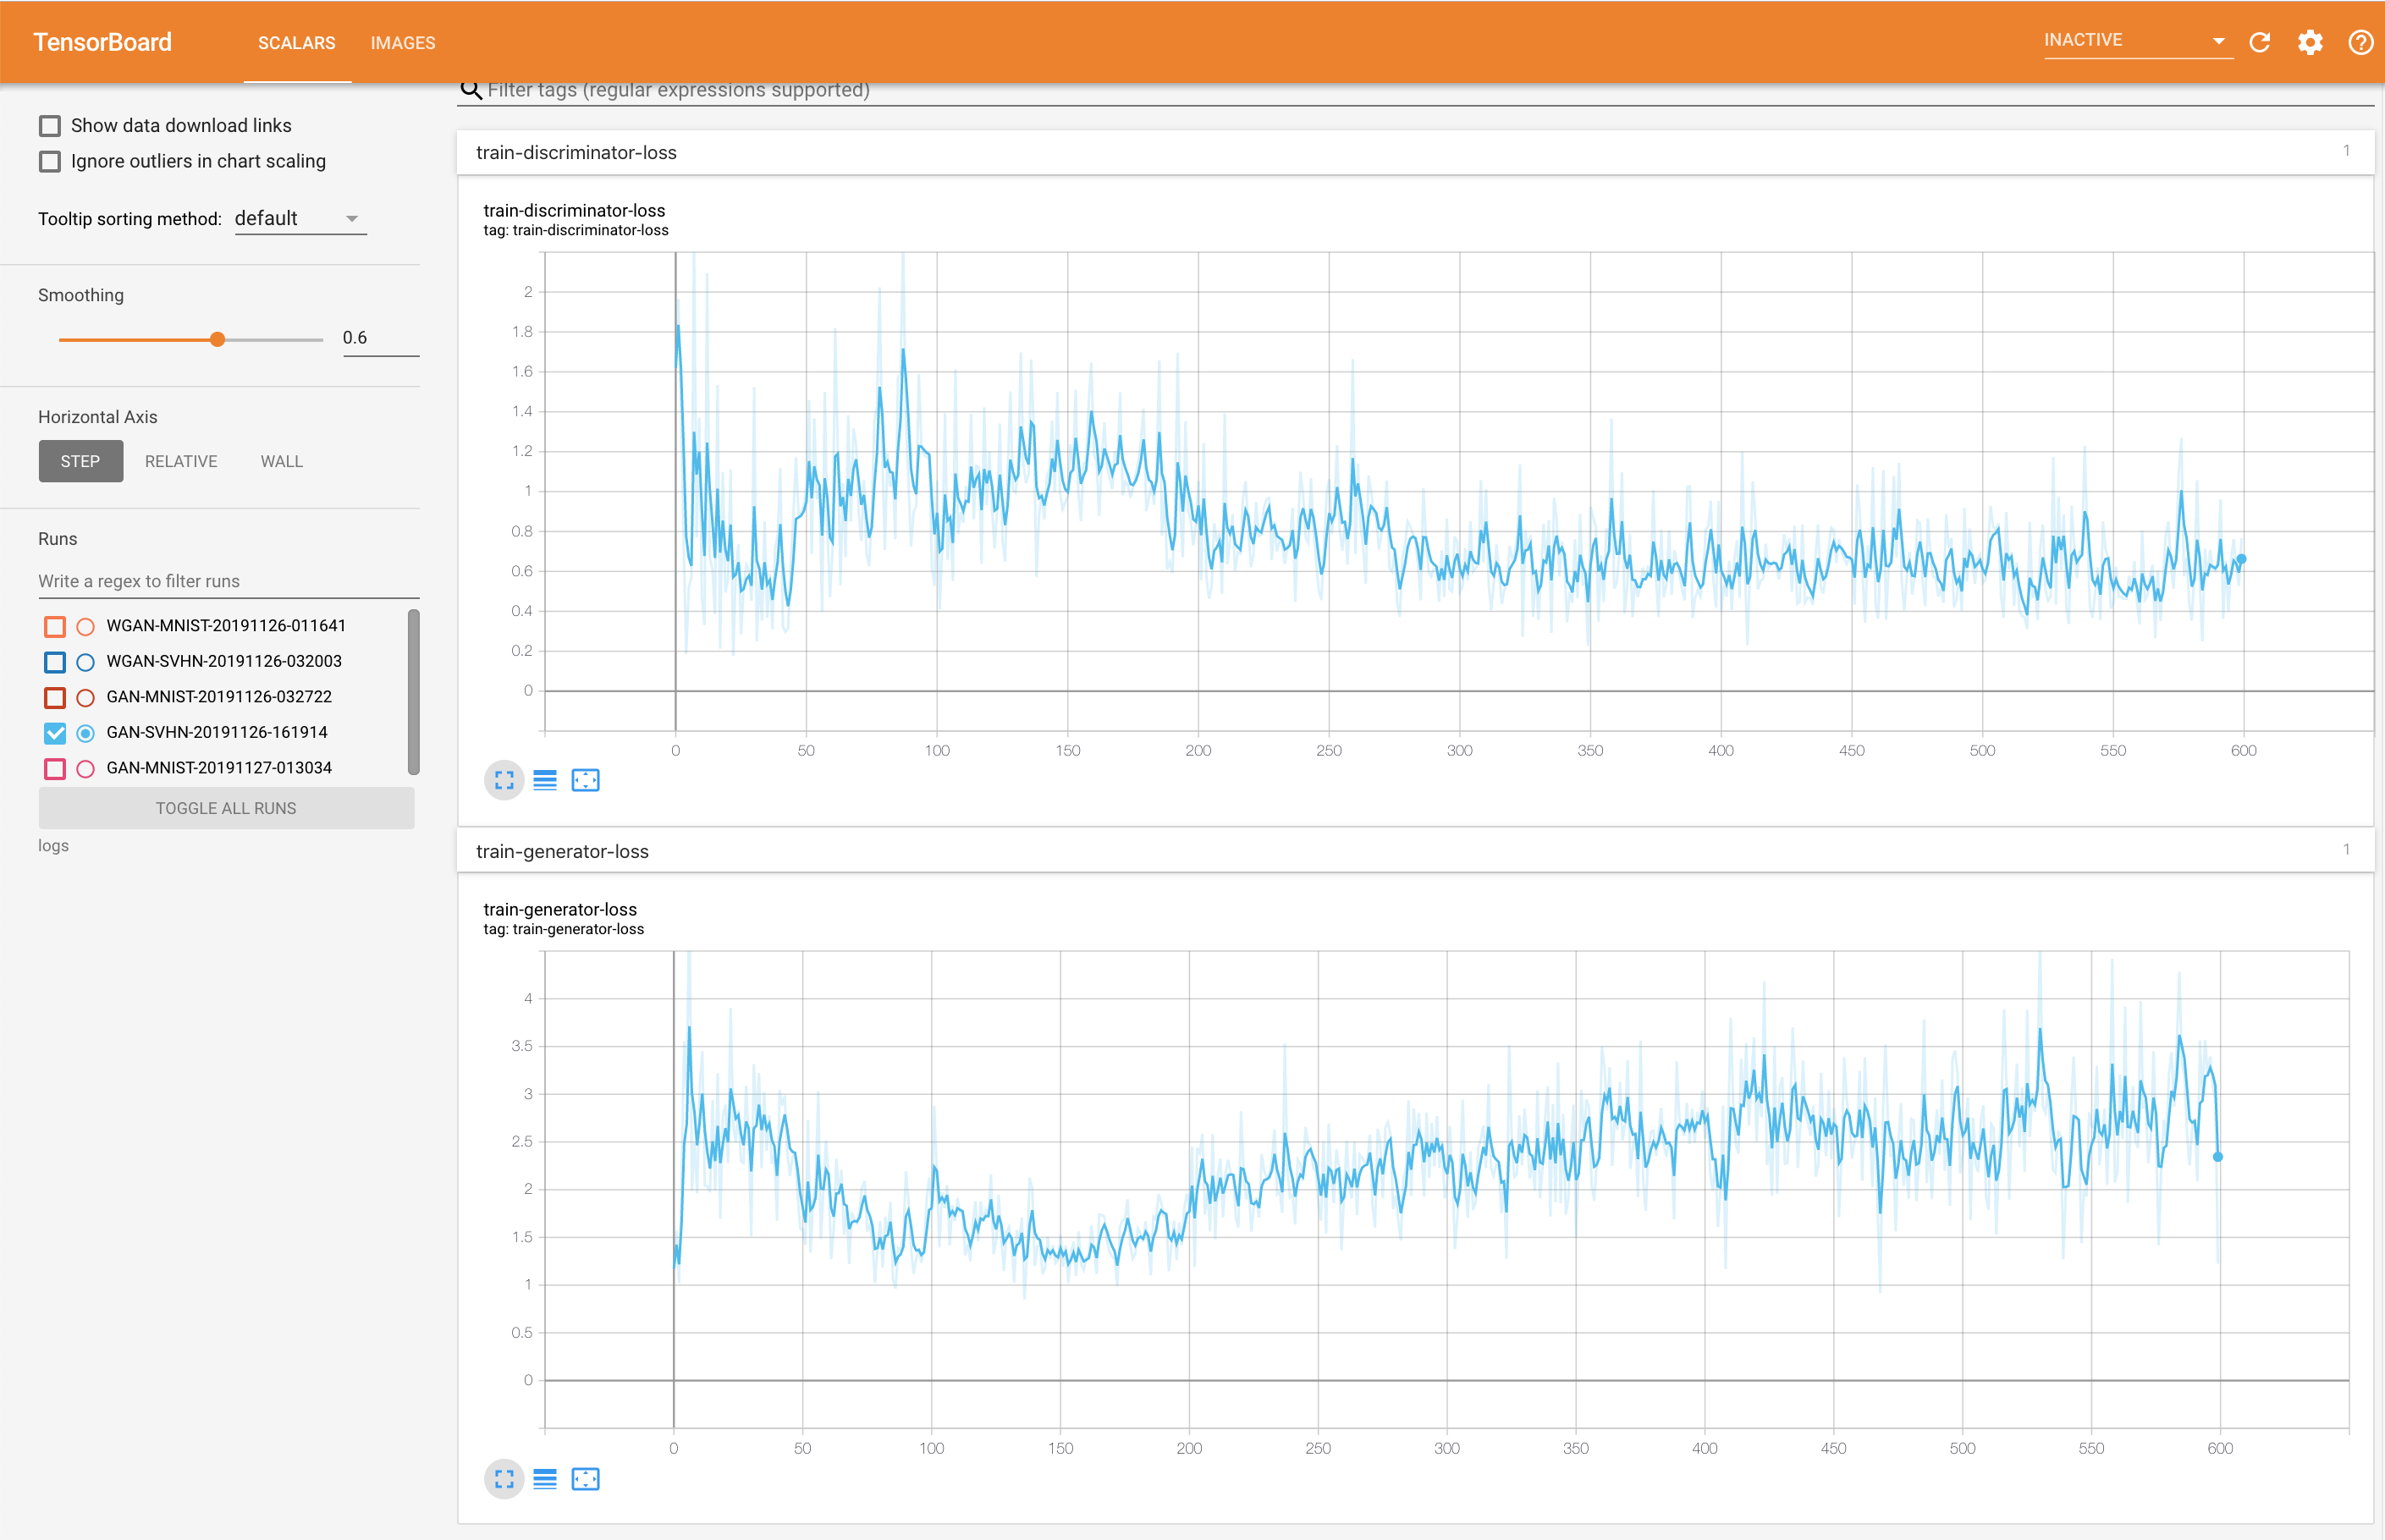
\includegraphics[width=0.8\textwidth]{tensorboard-GAN-SVHN.png}
  \caption{Tensorboard GAN SVHN}
  \label{fig:TB_GAN_SVHN}
\end{figure}

\subsubsection{Generated samples}

\begin{figure}[!htb]
  \centering
  \subfloat[SVHN data]{
  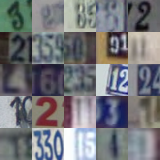
\includegraphics[width=0.2\textwidth]{svhn_data.png}}
  \subfloat[Epoch 30/200]{
  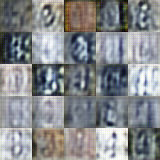
\includegraphics[width=0.2\textwidth]{s1_after-103-batches.png}}
  \subfloat[Epoch 150/200]{
  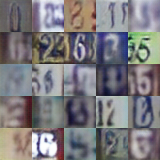
\includegraphics[width=0.2\textwidth]{s2_after-514-batches.png}}
  \subfloat[Epoch 200/200]{
  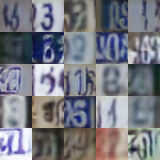
\includegraphics[width=0.2\textwidth]{s3_after-590-batches.png}}
  \caption{Comparison of SVHN data and generated samples from DCGAN}
  \label{fig:DCGAN_SVHN}
\end{figure}

The quality of the generated samples are not as good as the MNIST samples since the SVHN dataset is more complicated.
This complexity makes the model harder to converge i.e. uses more epoches to get good generated samples.

Although complicated as the dataset is, the generated samples demonstrate some qualities such as the variety of the samples. There are different combinations of gree, white, and red background with white, blue, and red fonts.

\section{WGAN}

Wasserstein GAN is a modified GAN introduced by Arjovsky, Martin, et al.(2017)[5]. 
It proposed Wasserstein that has a better property than Jensen-Shannon divergence.

Down to the implementation, the main difference is the loss function. We modified the loss function from \textit{BinaryCrossentropy} to a customized loss function.

The generator and discriminator are exactly the same as the GAN.

The hyperparameters are the same except this time we only train 50 epoches for each model.

\subsection{WGAN on MNIST}

\begin{figure}[!htb]
  \centering
  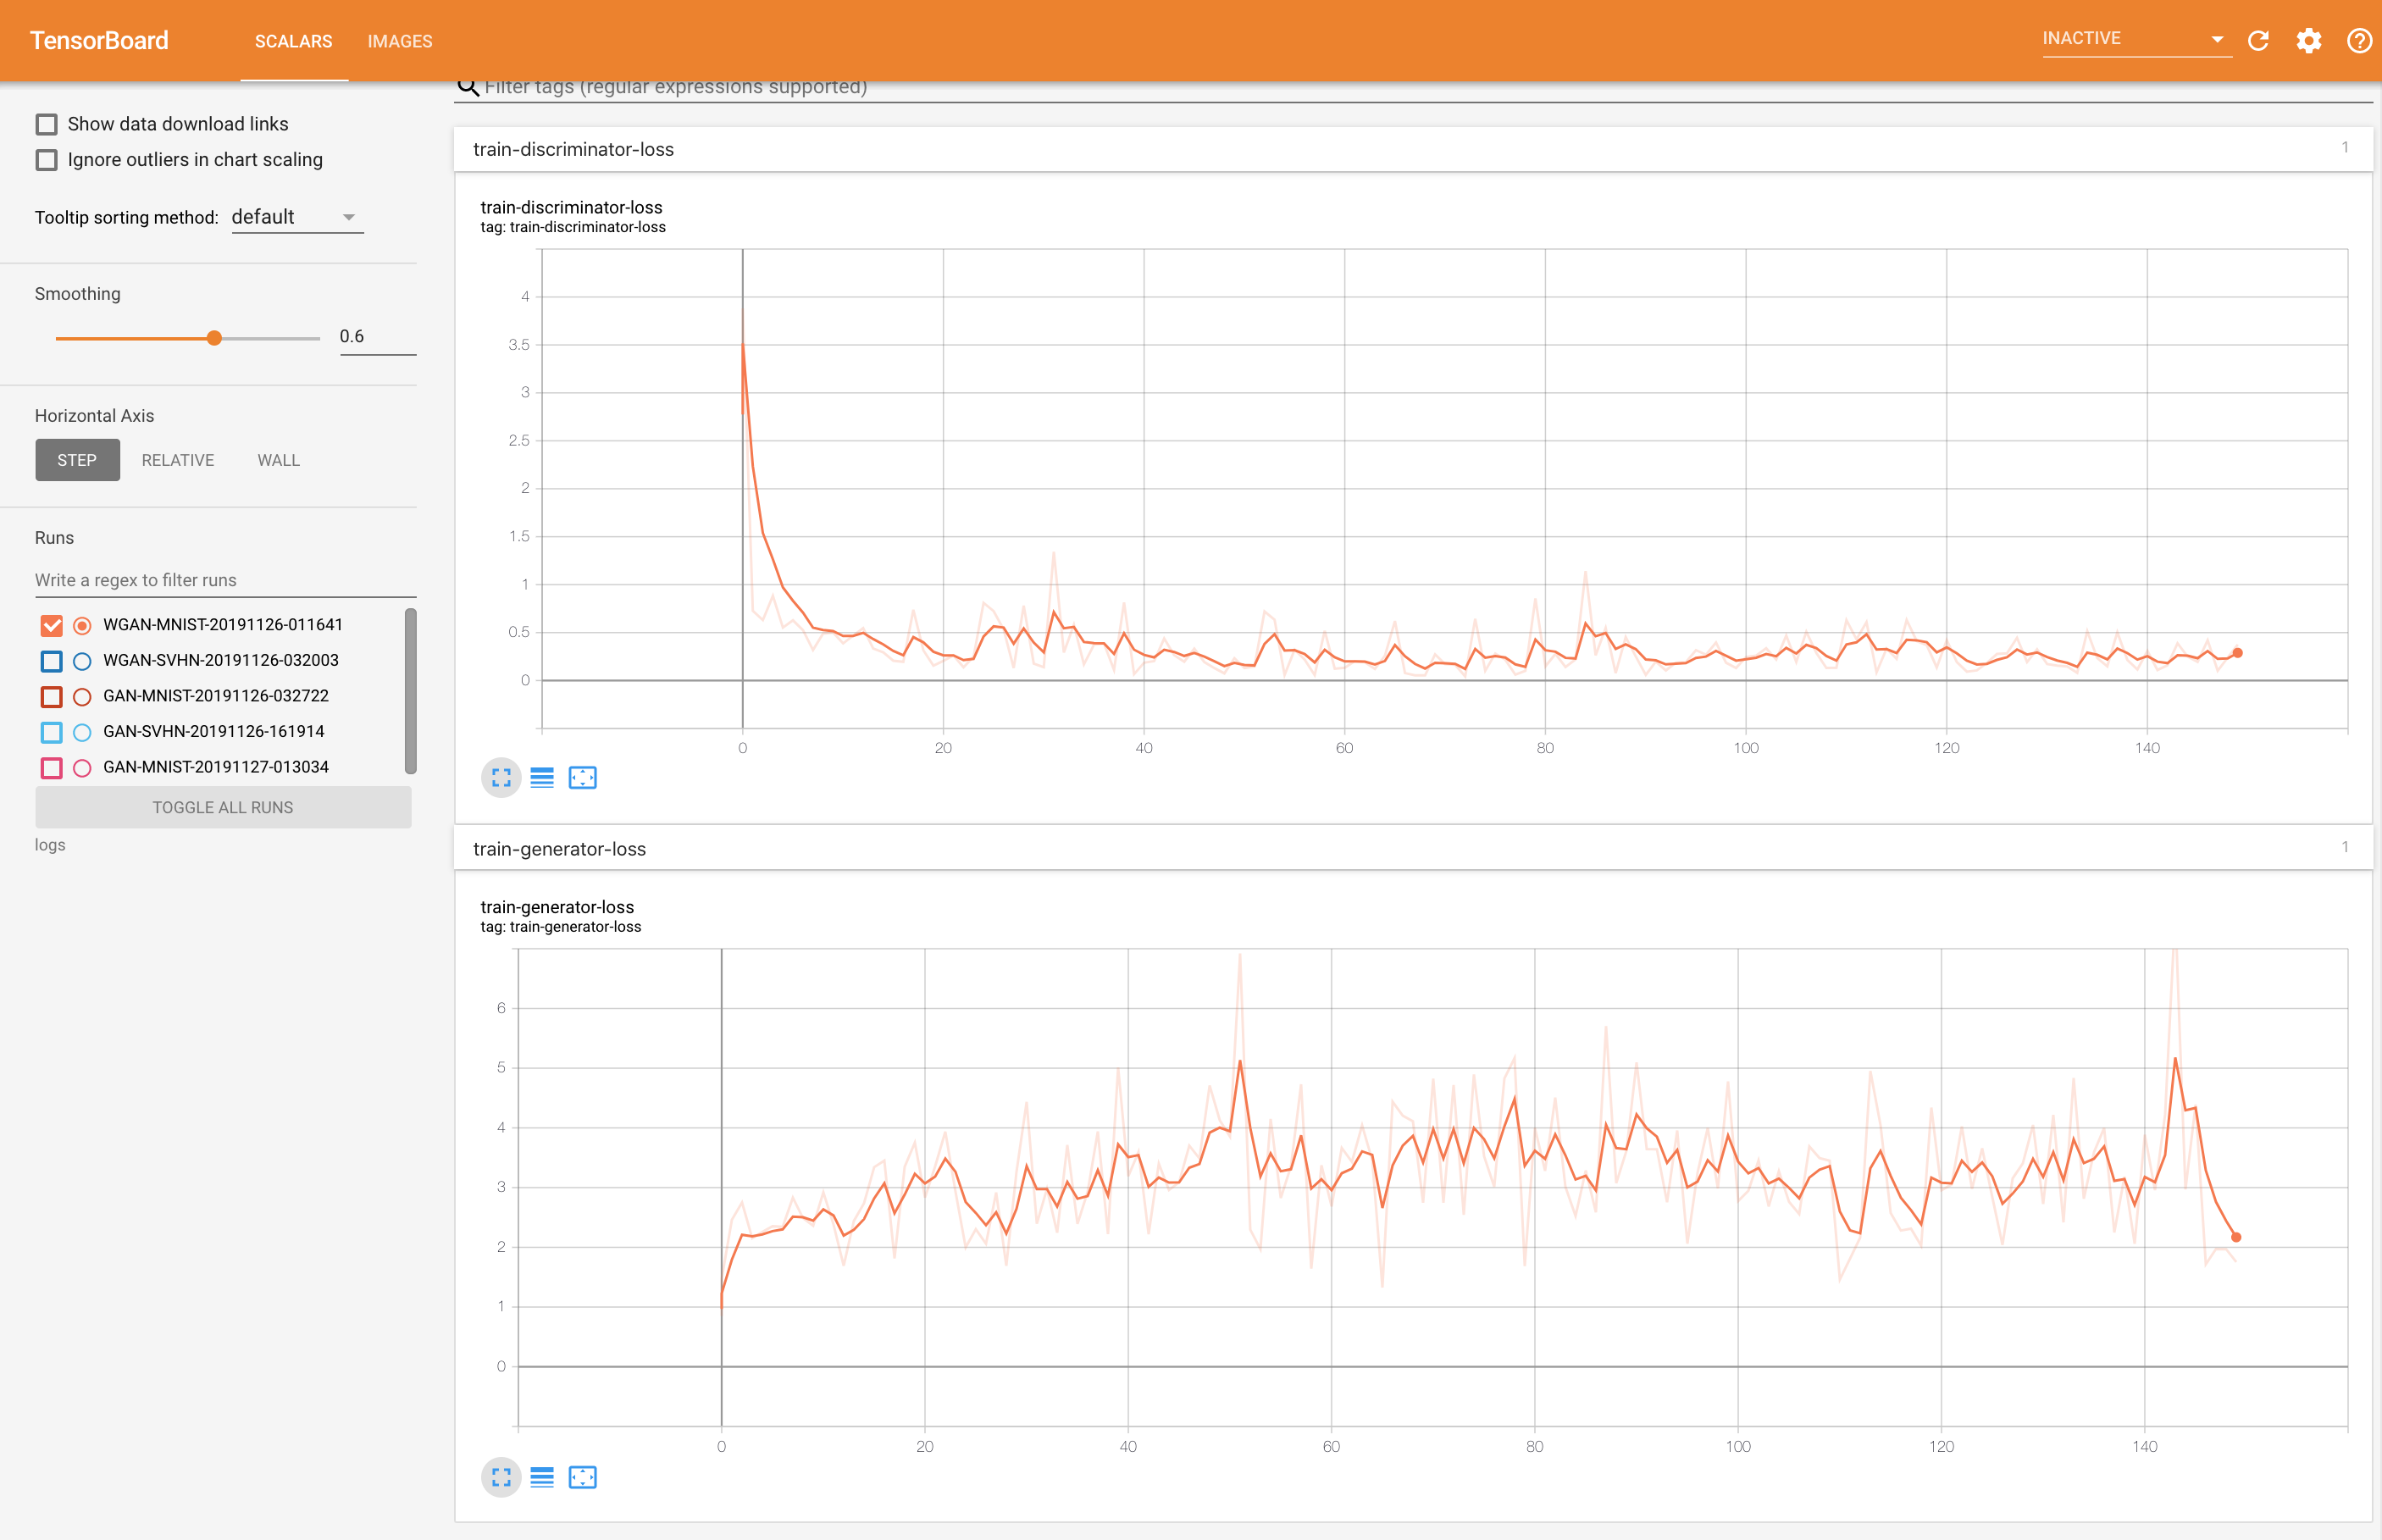
\includegraphics[width=0.8\textwidth]{tensorboard-WGAN-MNIST.png}
  \caption{Tensorboard WGAN MNSIT}
  \label{fig:TB_WGAN_MNSIT}
\end{figure}

\begin{figure}[!htb]
  \centering
  \subfloat[MNIST data]{
  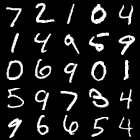
\includegraphics[width=0.2\textwidth]{mnist_data.png}}
  \subfloat[Epoch 10/50]{
  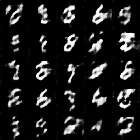
\includegraphics[width=0.2\textwidth]{I5_after-31-batches.png}}
  \subfloat[Epoch 30/50]{
  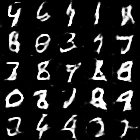
\includegraphics[width=0.2\textwidth]{I6_after-101-batches.png}}
  \subfloat[Epoch 50/50]{
  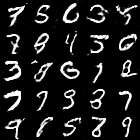
\includegraphics[width=0.2\textwidth]{I7_after-149-batches.png}}
  \caption{Comparison of MNIST data and generated samples from WGAN}
\end{figure}

\subsection{WGAN on SVHN}

\begin{figure}[!htb]
  \centering
  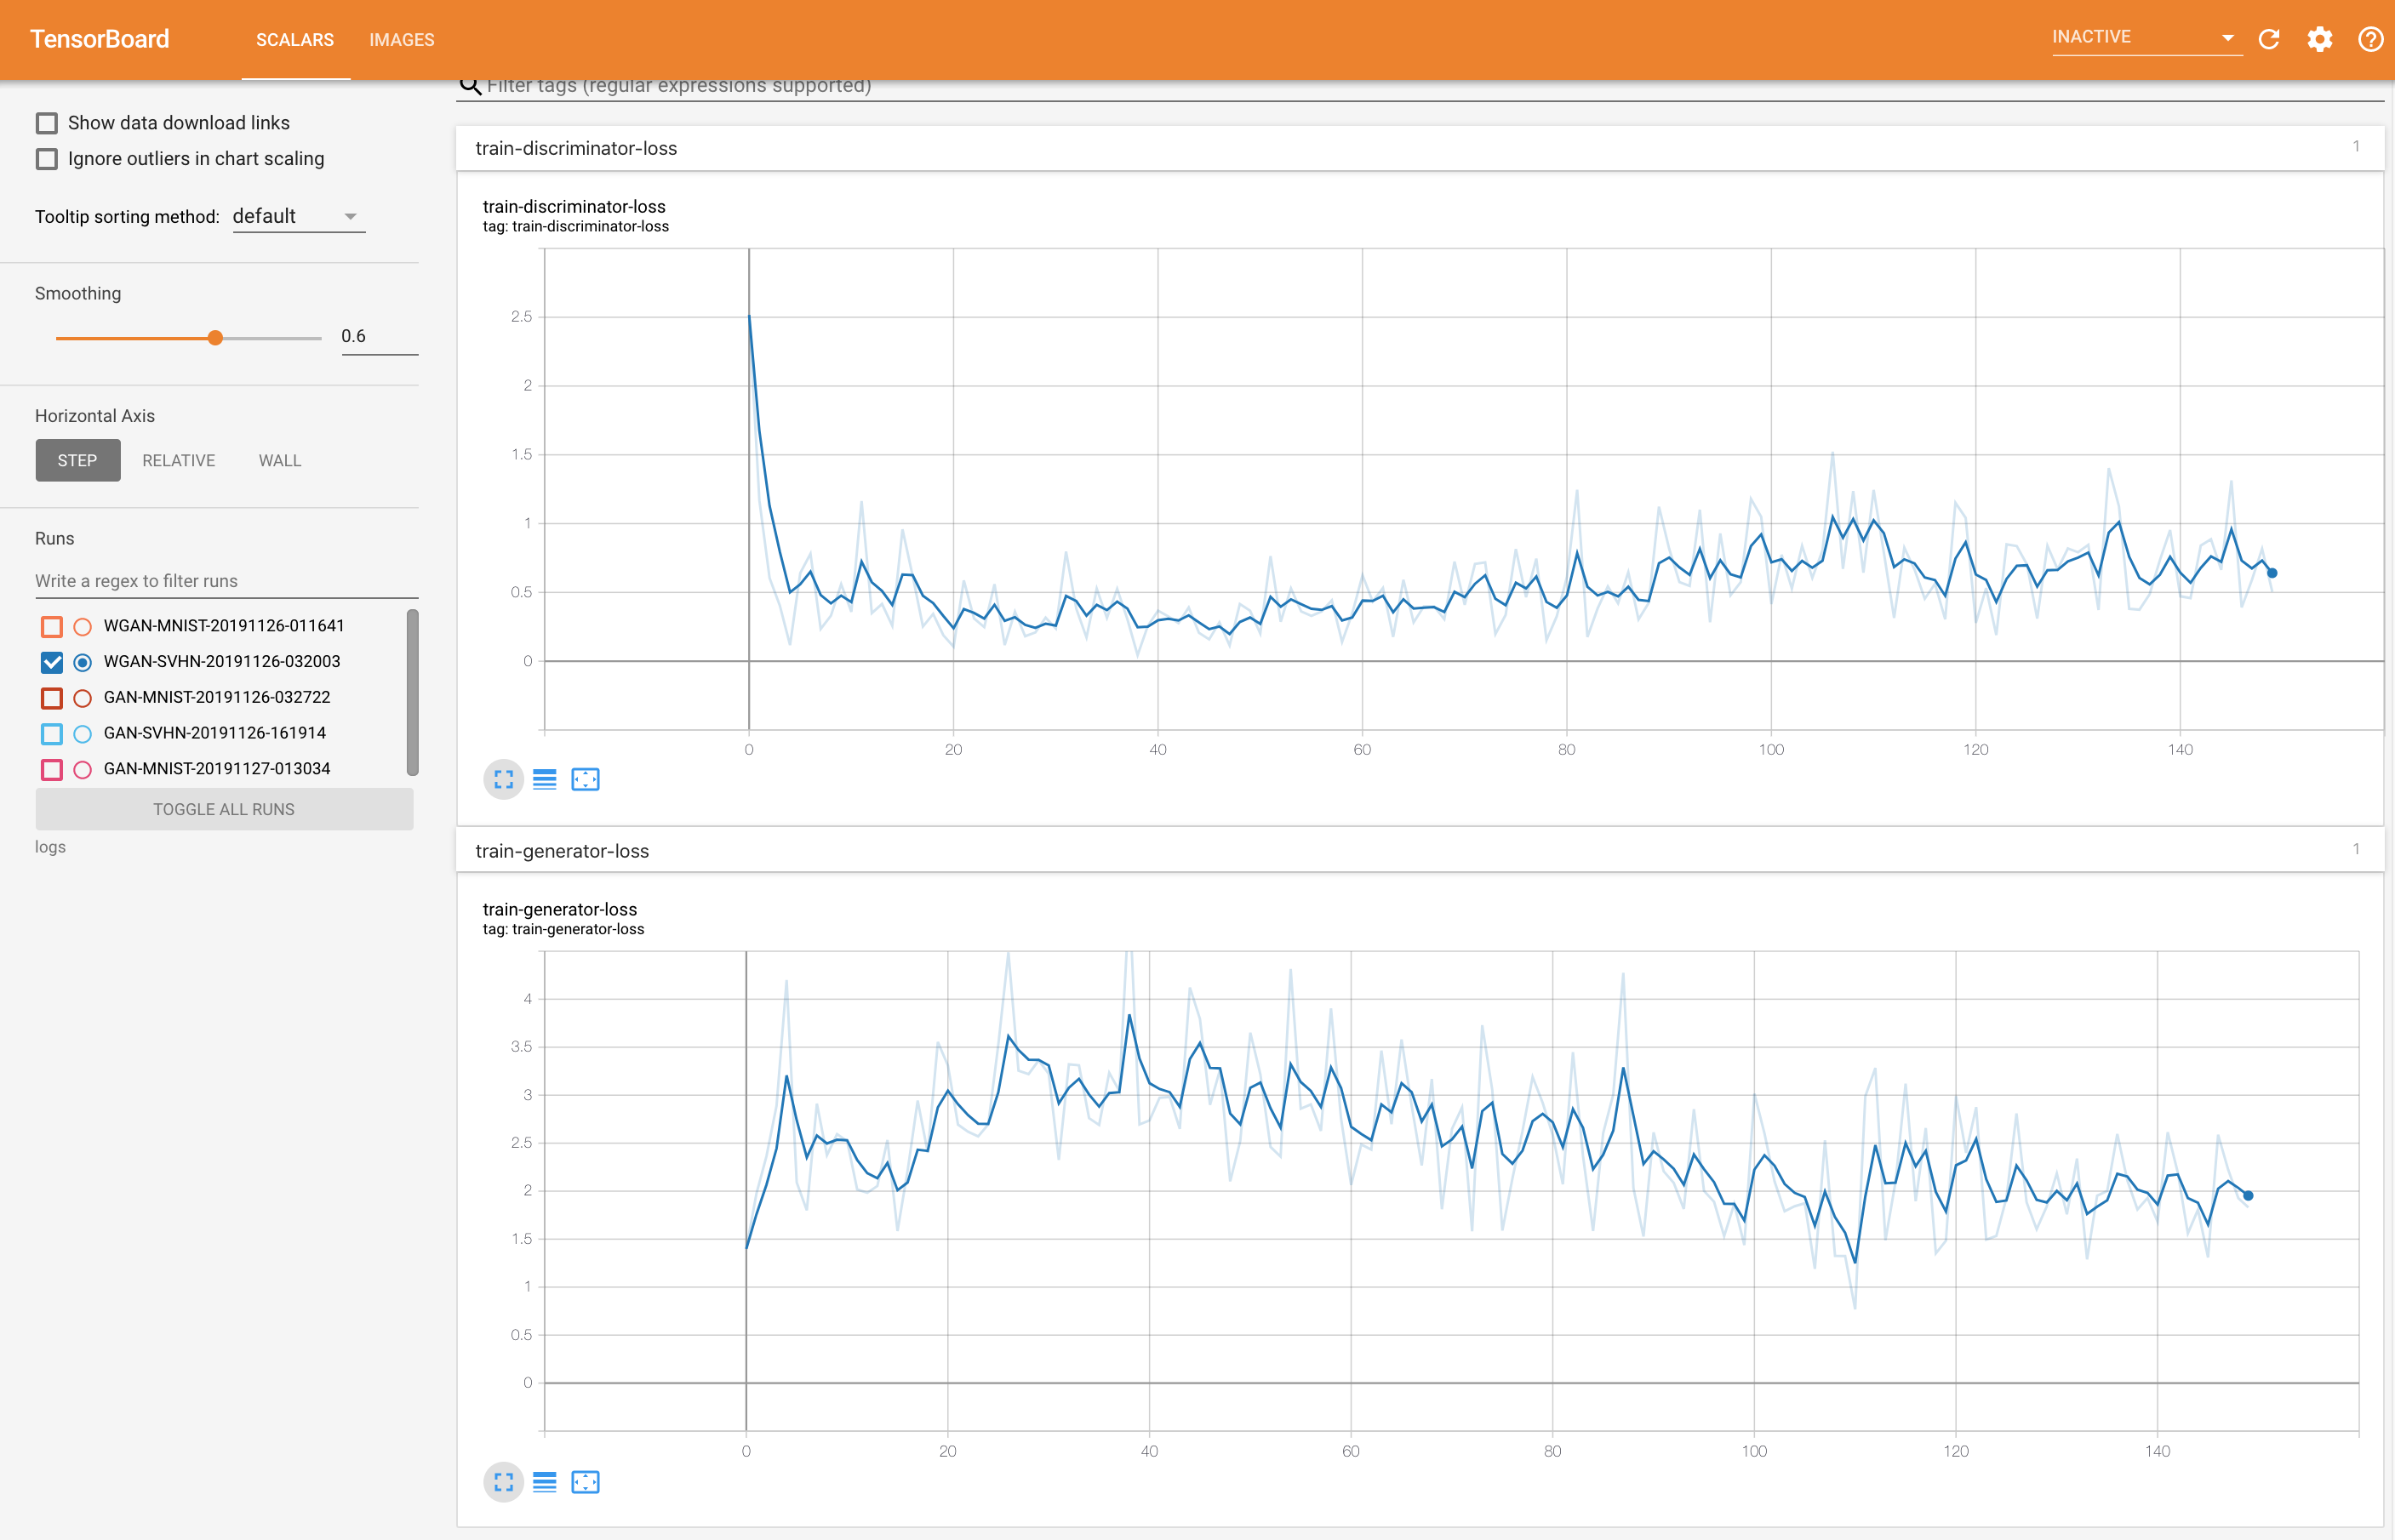
\includegraphics[width=0.8\textwidth]{tensorboard-WGAN-SVHN.png}
  \caption{Tensorboard WGAN SVHN}
  \label{fig:TB_WGAN_SVHN}
\end{figure}

\begin{figure}[!htb]
  \centering
  \subfloat[SVHN data]{
  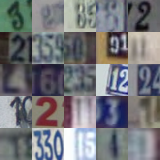
\includegraphics[width=0.2\textwidth]{svhn_data.png}}
  \subfloat[Epoch 10/50]{
  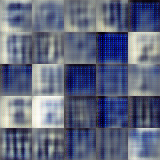
\includegraphics[width=0.2\textwidth]{s4_after-30-batches.png}}
  \subfloat[Epoch 30/50]{
  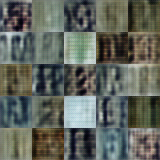
\includegraphics[width=0.2\textwidth]{s5_after-102-batches.png}}
  \subfloat[Epoch 50/50]{
  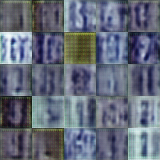
\includegraphics[width=0.2\textwidth]{s6_after-142-batches.png}}
  \caption{Comparison of SVHN data and generated samples from WGAN}
\end{figure}

\section{Summary}

xxx

\subsection{Future steps}

Since plenty new models have been published other than WGAN, we can try other models such as triple-GAN, Self-attention neural network, etc..

\clearpage
\section*{References}

[1] Goodfellow, Ian, et al. "Generative adversarial nets." Advances in neural information processing systems. 2014.

[2] LeCun, Yann, et al. “THE MNIST DATABASE.” MNIST Handwritten Digit Database, http://yann.lecun.com/exdb/mnist/.

[3] Netzer, Yuval, et al. "Reading digits in natural images with unsupervised feature learning." (2011).

[4] Radford, Alec, Luke Metz, and Soumith Chintala. "Unsupervised representation learning with deep convolutional generative adversarial networks." arXiv preprint arXiv:1511.06434 (2015).

[5] Arjovsky, Martin, Soumith Chintala, and Léon Bottou. "Wasserstein gan." arXiv preprint arXiv:1701.07875 (2017).

\end{document}
